\documentclass[a4paper,12pt]{article}
% Package to make citations superscrit with brackets
\usepackage[super,square]{natbib}
% Package to change margin size
\usepackage{anysize}
\usepackage{amsmath}
\marginsize{2cm}{2cm}{1cm}{2cm}
% Package to make headers
\usepackage{fancyhdr}
\usepackage{circuitikz}
\renewcommand{\headrulewidth}{0pt}
\usepackage{soul}
\usepackage[section]{placeins}
% Colors for the references links
\usepackage[dvipsnames]{xcolor}
% Package to link references
\usepackage{hyperref}
\usepackage{graphicx}
\hypersetup{
    colorlinks=true,
    linkcolor=black,
    citecolor=CadetBlue,
    filecolor=CadetBlue,      
    urlcolor=CadetBlue,
}
% Package for lorem ipsum
\usepackage{lipsum}
% Package for multicolumn
\usepackage{multicol}
% Package for removing paragraph identations
\usepackage{parskip}
\setlength\columnsep{18pt}
% Sets bastract
\renewenvironment{abstract}
 {\par\noindent\textbf{\abstractname}\ \ignorespaces \\}
 {\par\noindent\medskip}



 
\begin{document}
% Makes header
\pagestyle{fancy}
\thispagestyle{empty}
\fancyhead[R]{\textit{EE1200}}
\fancyhead[L]{}
% Makes footnotes with an asterisk
\renewcommand*{\thefootnote}{\fnsymbol{footnote}}
\begin{center}
\Large{\textbf{Experiment 02}}
\vspace{0.4cm}
\normalsize
\\ Aditya Tripathy - ee24btech11001, Durgi Swaraj Sharma - ee24btech11018\\
\medskip
\normalsize
\end{center}
{\color{gray}\hrule}
\vspace{0.4cm}
\begin{abstract}
In Experiment-02, we studied the response of an RC circuit to a square wave input for different ranges of the time constant.
\end{abstract}
{\color{gray}\hrule}
\medskip
\section{Objective}
To study the response of RC circuit to square wave input voltage signal when 
\begin{enumerate}
  \item RC = T
  \item RC $>>$ T
  \item RC $<<$ T
\end{enumerate}
\section{Apparatus}
\begin{itemize}
\item Oscilloscope
\item Two channel function generator
\item Connecting wires and probes
\item Unpolarised capacitor (0.1$\mu$F)
\item Resistors(100$\Omega$, 1k$\Omega$, 10k$\Omega$, 1M$\Omega$)
\end{itemize}
\section{Theory}
\begin{figure}[!ht]
\centering
\resizebox{0.5\textwidth}{!}{%
\begin{circuitikz}
\tikzstyle{every node}=[font=\LARGE]
\draw (11,11.5) to[square voltage source, sources/symbol/rotate=auto] (13,11.5);
\draw (11,11.5) to[short] (9.25,11.5);
\draw (9.25,11.5) to[short] (9.25,14.25);
\draw (13,11.5) to[short] (15.25,11.5);
\draw (15.25,11.5) to[short] (15.25,14.5);
\draw (9.25,14.25) to[R] (13.5,14.25);
\draw (12,14.25) to[C] (15.25,14.25);
\draw (12.75,14.25) to[short, -o] (12.75,15.5) ;
\draw (15.25,14.25) to[short, -o] (15.25,15.5) ;
\node [font=\LARGE] at (9.25,16) {A};
\draw (15.25,14.25) to (15.25,10.55) node[ground]{};
\node [font=\LARGE] at (15,16.5) {};
\node [font=\LARGE] at (12.75,16) {B};
\draw (9.25,14.25) to[short, -o] (9.25,15.5) ;
\node [font=\LARGE] at (15.25,16) {C};
\end{circuitikz}
}%
\label{fig:my_label}
\end{figure}
The voltage across capacitor is governed by the following differential equation,
\begin{align}
  V(t) = RC\frac{dV_C}{dt} + V_C\\
  \Rightarrow \frac{dV_C}{dt} = \frac{1}{RC}(V(t) - V_C)
\end{align}
This can be solved numerically using trapezoidal rule, 
\begin{align}
  V(t_{n+1}) = V(t_n) + \frac{h}{2RC}(V(t_{n+1}) + V(t_n) - V_C(t_{n+1}) - V_C(t_n))\\
  V(t_{n+1}) = V(t_n)\left( \frac{2RC-h}{2RC+h}\right) + \frac{h}{2RC+h}(V(t_{n+1})+V(t_n))
\end{align}
Now the aim is to study experimental response in the three aforementioned cases in light of theoretical solution.
\section{Procedure}
\begin{enumerate}
\item Connections
\begin{itemize}
\item Connect the first channel of the function generator to terminal A, and associated ground to C.
\item Connect the first channel of the oscilloscope to terminal A, and the associated ground to C.
\item Connect the second channel of the oscilloscope to terminal B, and the associated ground to C.
\item Ensure scaling is 10X both on the probe wires and the oscilloscope.
\end{itemize}
\item Device Setup
\begin{itemize}
\item Construct the circuit as shown in the figure above.
\item Use appropriate values of the components for the tree separate cases.
\item Use the square wave output function in the function generator and use the Time Period option to set the desired time period for the voltage signal.
\item To capture the response to first few cycles of input voltage signal, set an appropriate trigger level, set "Sweep = Normal" under "Mode Coupling" menu and set "Trigger = Manual" on the function generator.
\end{itemize}
\item Make sure that you either use an unpolarised capacitor, with an input voltage signal with
  high of 5Vrms and low value of -5Vrms, or use an electrolytic capacitor with same high value but 
  low value of 0mV with the longer terminal of the capacitor connected to higher potential.
\end{enumerate}
\section{Justification}
We will be using Python along with Matplotlib and Numpy libraries to verify our experiment's results. The following code plots out the theoretical response of the RC circuit to the input square wave using the numerical solution shown above.
\begin{verbatim}
import matplotlib.pyplot as plt 
import numpy as np 

def V(t, T, A):
    if t % T <= T/2:
        return A 
    else :
        return 0

h = 1e-6
V_0 = 0
t_0 = 0
def f(R, C, V, t, A, T):
    return V(t, A, T)/(R * C) - V/(R*C*C)
R = 1e4
C = 1e-7
A = 5
T = 1
print("T = ", T)
print("RC = ", R*C)
time = list()
V_vals = list()
num_points = 1000000
for _ in range(num_points):
    time.append(t_0)
    V_vals.append(V_0)
    V_0 = V_0 * (2*R*C - h)/(2*R*C +h) +  h/(2*R*C + h) * (V(t_0, T, A) + V(t_0 + h, T, A))
    t_0 += h
plt.plot(time, V_vals)
plt.xlim(0, 0.1)
plt.ylim(-5.2, 5.2)
plt.savefig("RC=T.png")
plt.show()
\end{verbatim}
By following the procedure for different values R and C, we produced the following  verified them using the previously mentioned code.
The parameters for the signals used are present in the pictures.
\section{Results}
\begin{figure}[!htb]
  {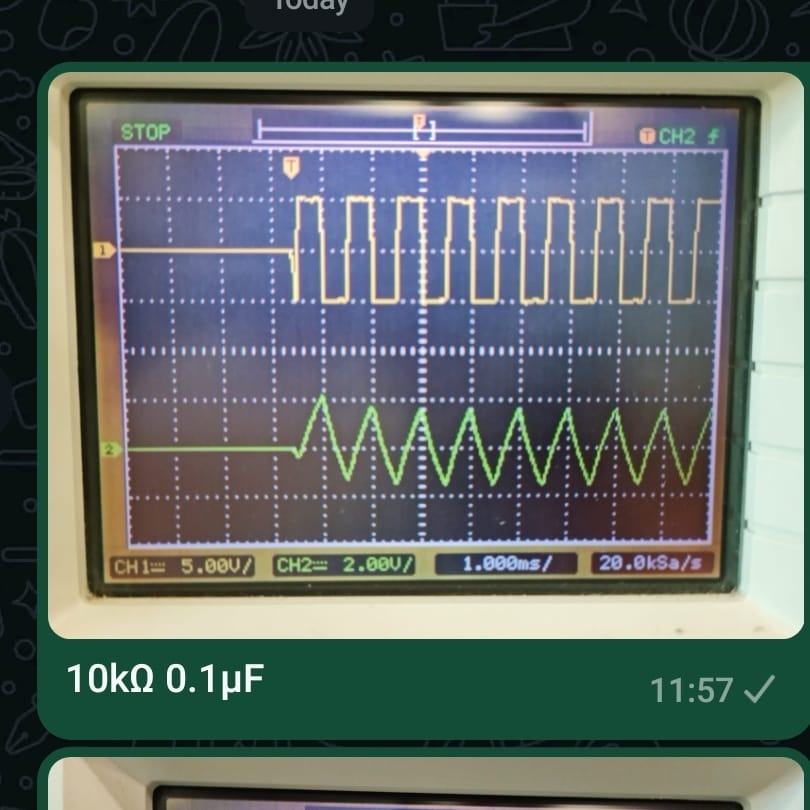
\includegraphics[width=0.5\columnwidth]{figs/RC=T_exp.jpg}}
  \hspace{\fill}
  {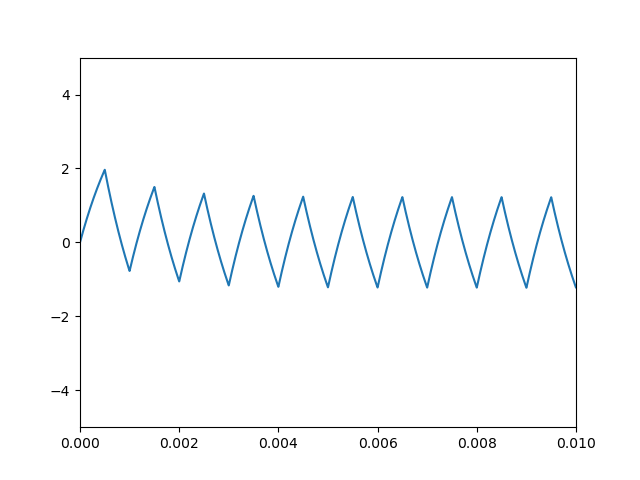
\includegraphics[width=0.5\columnwidth]{figs/RC=T_sim.png}}
  \caption{RC = T}
\end{figure}
 \begin{figure}[!htb]
  {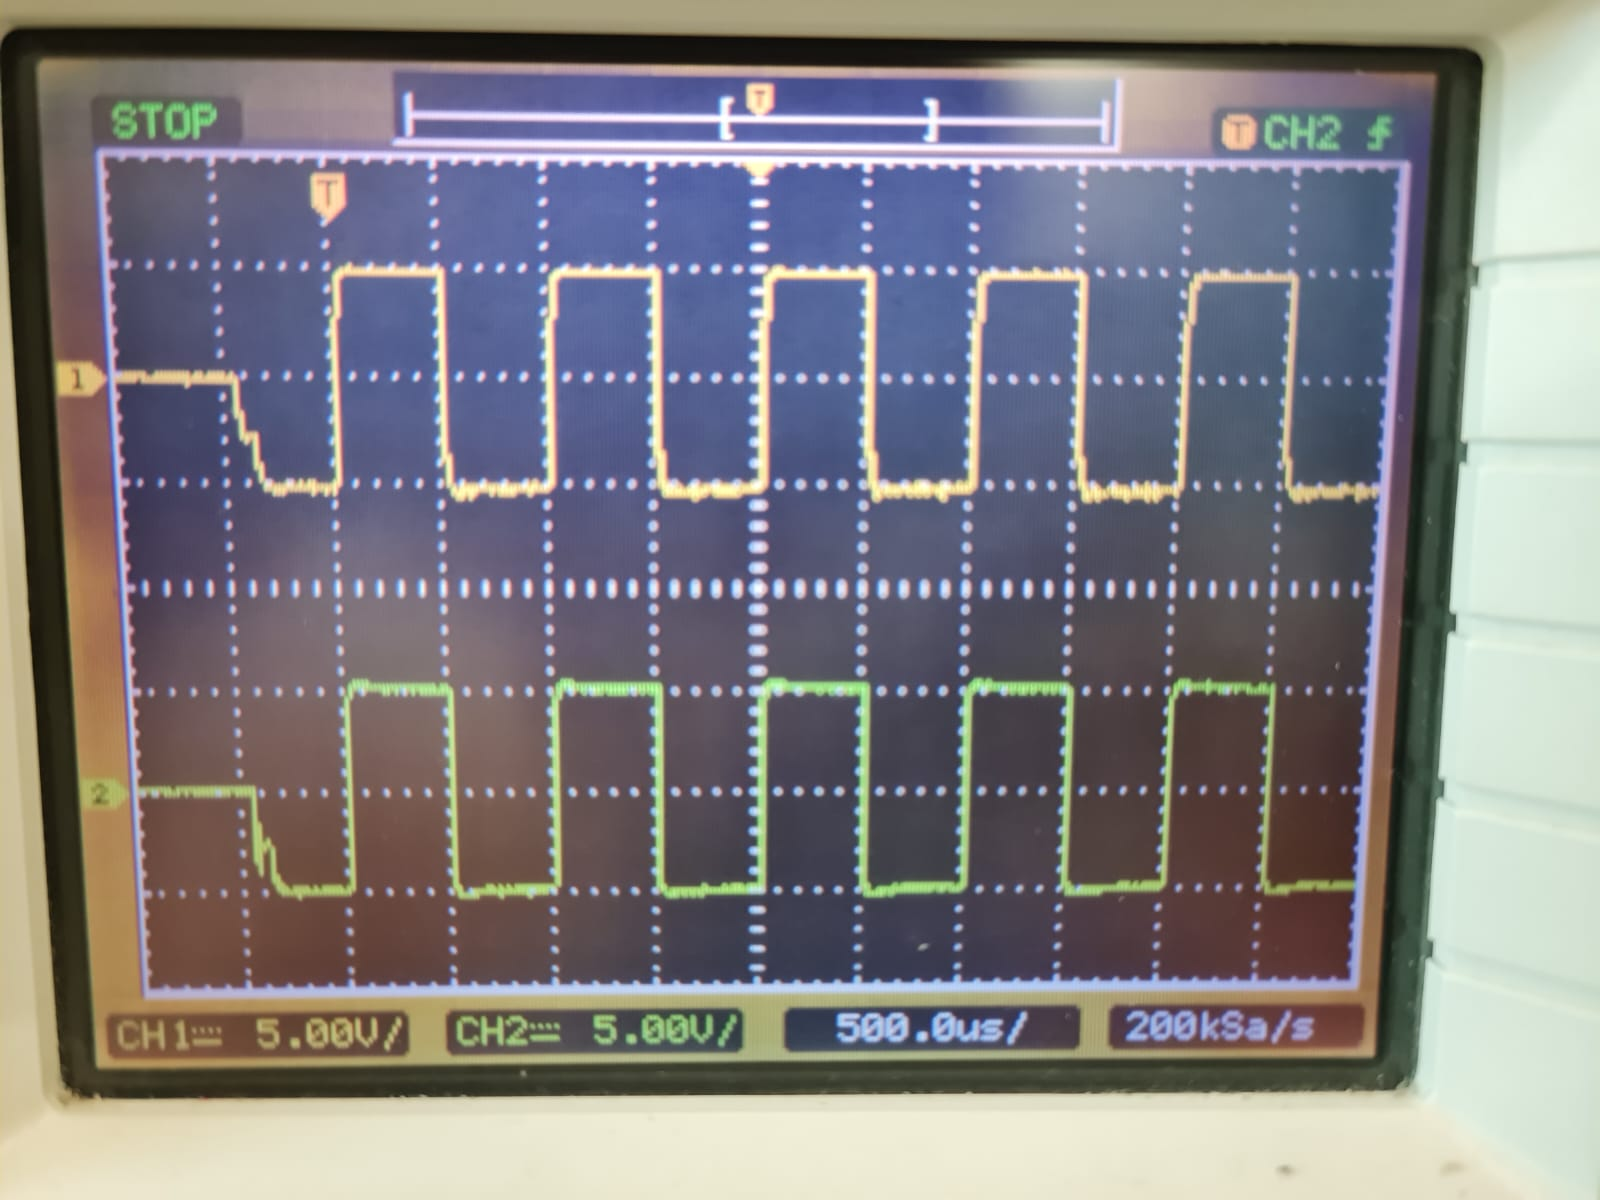
\includegraphics[width=0.5\columnwidth]{figs/RC=0.01T_exp.jpg}}
  \hspace{\fill}
  {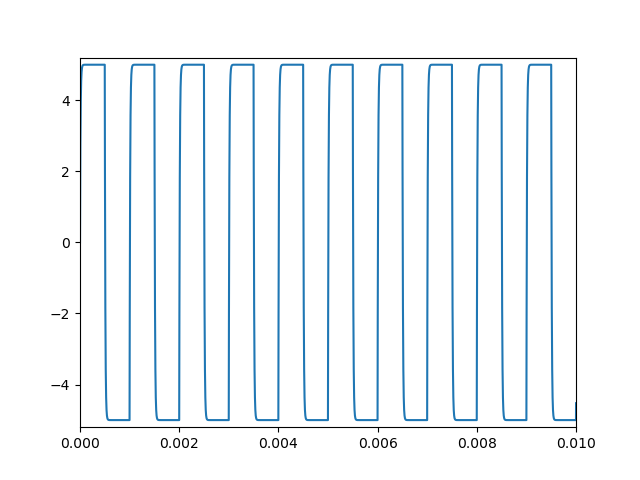
\includegraphics[width=0.5\columnwidth]{figs/RC=0.01T_sim.png}}
  \caption{RC = 0.01T}
\end{figure}
\begin{figure}[!htb]
  {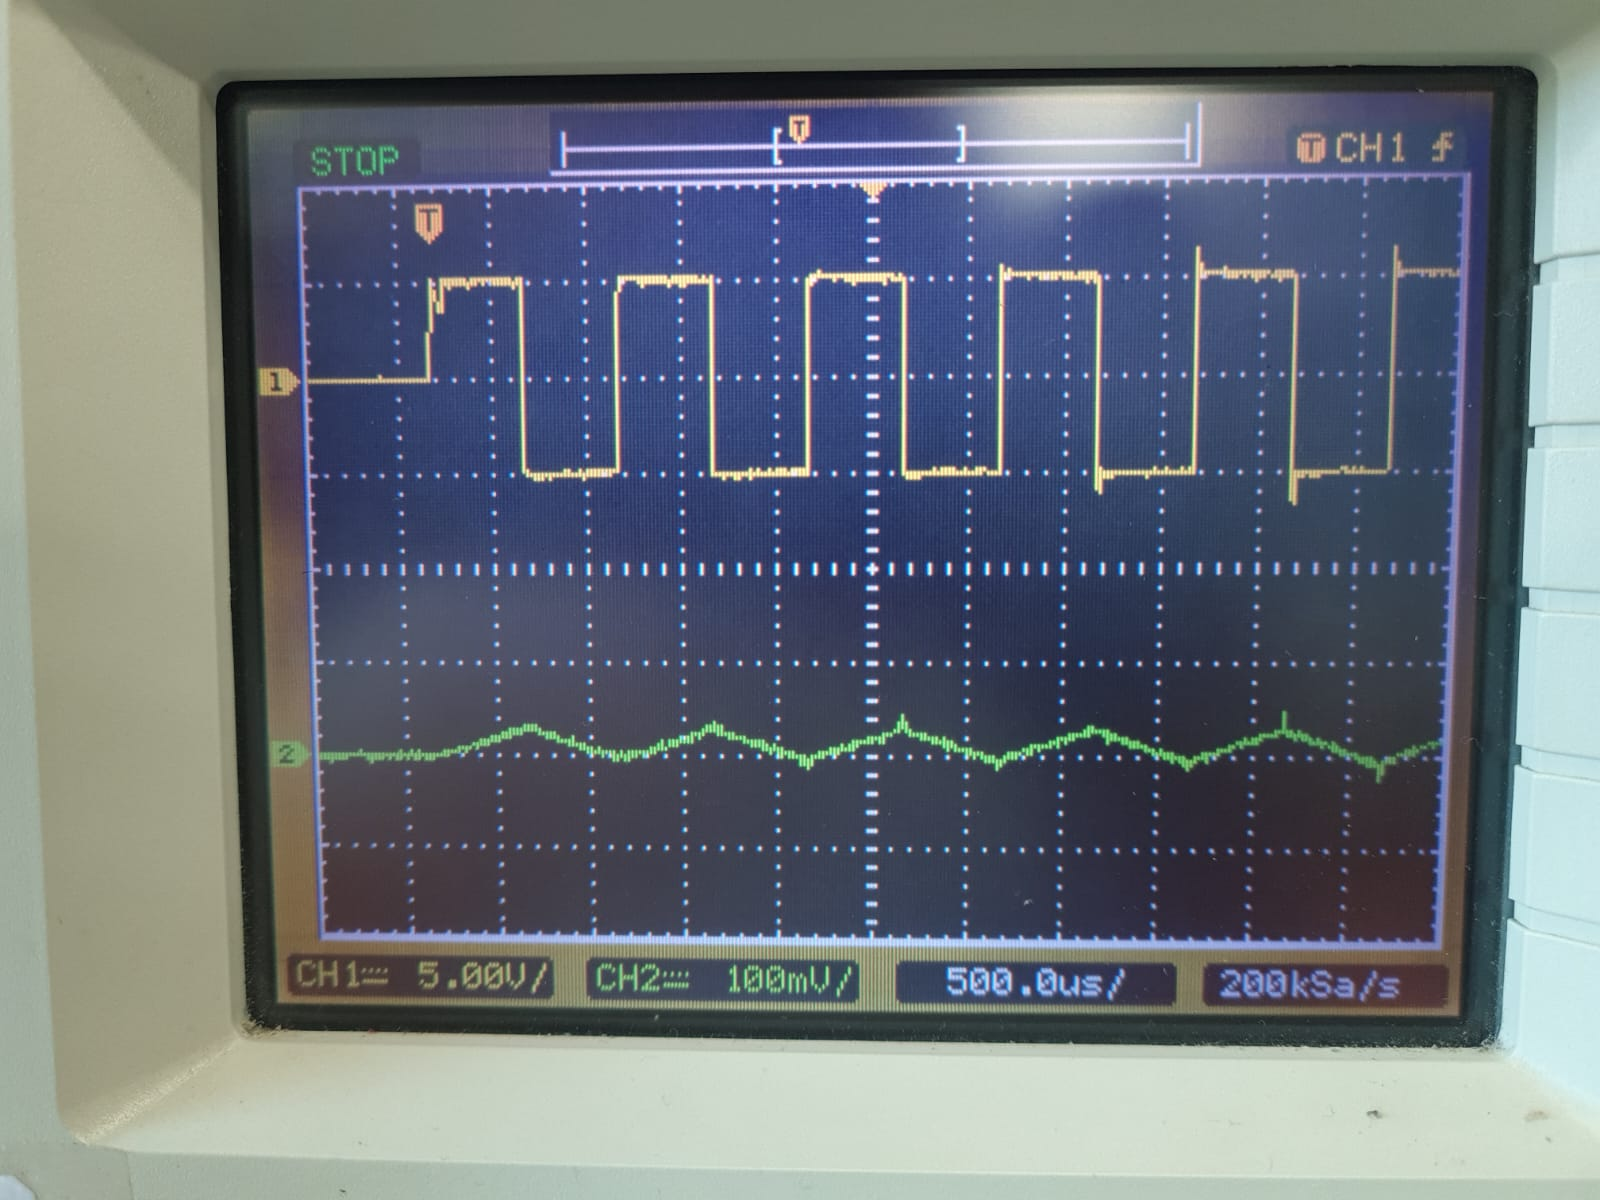
\includegraphics[width=0.5\columnwidth]{figs/RC=100T_exp.jpg}}
  \hspace{\fill}
  {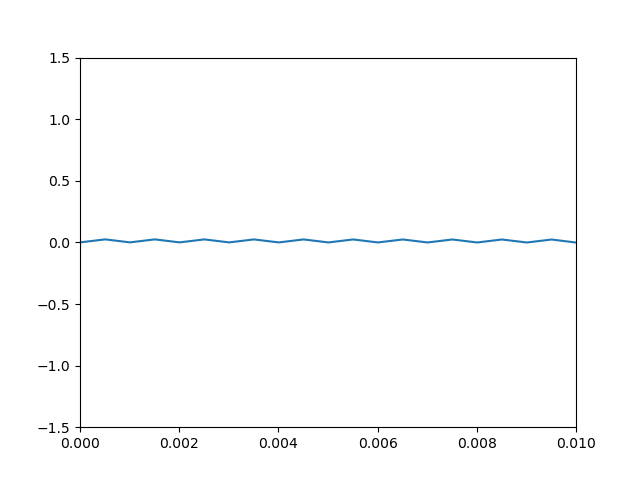
\includegraphics[width=0.5\columnwidth]{figs/RC=100T_sim.png}}
  \caption{RC = 100T}
\end{figure}
	\section{Conclusion}
We successfully graphed the response of an RC circuit to a square wave response.
\end{document}
